% Created by tikzDevice version 0.12.6 on 2025-11-06 20:50:33
% !TEX encoding = UTF-8 Unicode
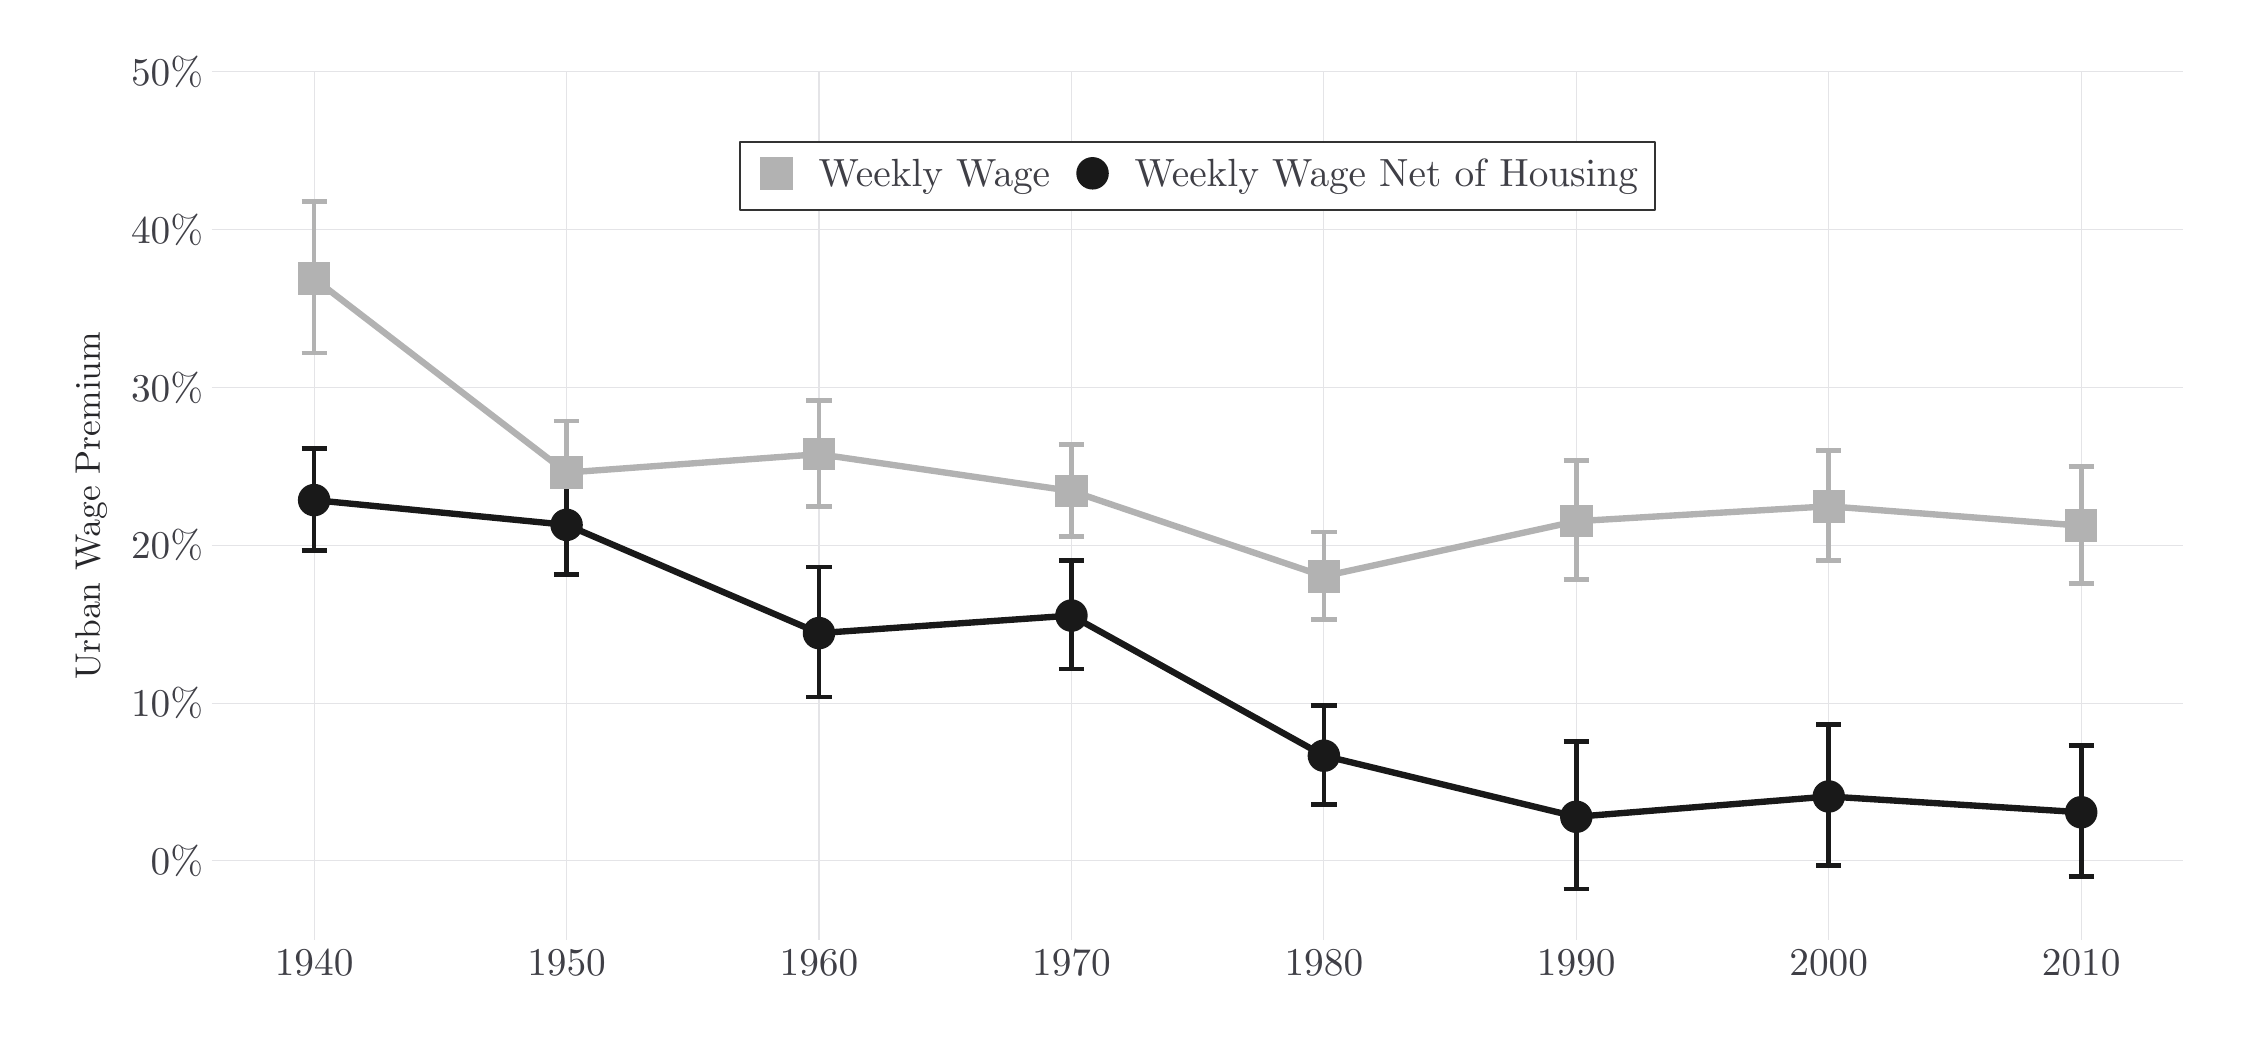
\begin{tikzpicture}[x=1pt,y=1pt]
\definecolor{fillColor}{RGB}{255,255,255}
\path[use as bounding box,fill=fillColor] (0,0) rectangle (794.97,361.35);
\begin{scope}
\path[clip] (  0.00,  0.00) rectangle (794.97,361.35);
\definecolor{drawColor}{RGB}{255,255,255}

\path[draw=drawColor,line width= 0.8pt,line join=round,line cap=round,fill=fillColor] (  0.00,  0.00) rectangle (794.97,361.35);
\end{scope}
\begin{scope}
\path[clip] ( 66.57, 31.76) rectangle (778.97,345.35);
\definecolor{drawColor}{RGB}{255,255,255}
\definecolor{fillColor}{RGB}{255,255,255}

\path[draw=drawColor,line width= 0.8pt,line join=round,line cap=round,fill=fillColor] ( 66.57, 31.76) rectangle (778.97,345.35);
\definecolor{drawColor}{RGB}{228,228,231}

\path[draw=drawColor,line width= 0.4pt,line join=round] ( 66.57, 60.27) --
	(778.97, 60.27);

\path[draw=drawColor,line width= 0.4pt,line join=round] ( 66.57,117.28) --
	(778.97,117.28);

\path[draw=drawColor,line width= 0.4pt,line join=round] ( 66.57,174.30) --
	(778.97,174.30);

\path[draw=drawColor,line width= 0.4pt,line join=round] ( 66.57,231.32) --
	(778.97,231.32);

\path[draw=drawColor,line width= 0.4pt,line join=round] ( 66.57,288.33) --
	(778.97,288.33);

\path[draw=drawColor,line width= 0.4pt,line join=round] ( 66.57,345.35) --
	(778.97,345.35);

\path[draw=drawColor,line width= 0.4pt,line join=round] (103.51, 31.76) --
	(103.51,345.35);

\path[draw=drawColor,line width= 0.4pt,line join=round] (194.73, 31.76) --
	(194.73,345.35);

\path[draw=drawColor,line width= 0.4pt,line join=round] (285.94, 31.76) --
	(285.94,345.35);

\path[draw=drawColor,line width= 0.4pt,line join=round] (377.16, 31.76) --
	(377.16,345.35);

\path[draw=drawColor,line width= 0.4pt,line join=round] (468.38, 31.76) --
	(468.38,345.35);

\path[draw=drawColor,line width= 0.4pt,line join=round] (559.59, 31.76) --
	(559.59,345.35);

\path[draw=drawColor,line width= 0.4pt,line join=round] (650.81, 31.76) --
	(650.81,345.35);

\path[draw=drawColor,line width= 0.4pt,line join=round] (742.03, 31.76) --
	(742.03,345.35);
\definecolor{drawColor}{gray}{0.70}

\path[draw=drawColor,line width= 2.3pt,line join=round] (103.51,270.65) --
	(194.73,200.59) --
	(285.94,207.23) --
	(377.16,193.93) --
	(468.38,163.11) --
	(559.59,183.01) --
	(650.81,188.40) --
	(742.03,181.39);
\definecolor{drawColor}{gray}{0.10}

\path[draw=drawColor,line width= 2.3pt,line join=round] (103.51,190.64) --
	(194.73,181.69) --
	(285.94,142.57) --
	(377.16,148.91) --
	(468.38, 98.27) --
	(559.59, 76.21) --
	(650.81, 83.54) --
	(742.03, 77.84);
\definecolor{drawColor}{gray}{0.70}

\path[draw=drawColor,line width= 1.7pt,line join=round] ( 98.95,298.42) --
	(108.07,298.42);

\path[draw=drawColor,line width= 1.7pt,line join=round] (103.51,298.42) --
	(103.51,243.84);

\path[draw=drawColor,line width= 1.7pt,line join=round] ( 98.95,243.84) --
	(108.07,243.84);
\definecolor{drawColor}{gray}{0.10}

\path[draw=drawColor,line width= 1.7pt,line join=round] ( 98.95,209.33) --
	(108.07,209.33);

\path[draw=drawColor,line width= 1.7pt,line join=round] (103.51,209.33) --
	(103.51,172.44);

\path[draw=drawColor,line width= 1.7pt,line join=round] ( 98.95,172.44) --
	(108.07,172.44);
\definecolor{drawColor}{gray}{0.70}

\path[draw=drawColor,line width= 1.7pt,line join=round] (190.17,219.25) --
	(199.29,219.25);

\path[draw=drawColor,line width= 1.7pt,line join=round] (194.73,219.25) --
	(194.73,182.40);

\path[draw=drawColor,line width= 1.7pt,line join=round] (190.17,182.40) --
	(199.29,182.40);
\definecolor{drawColor}{gray}{0.10}

\path[draw=drawColor,line width= 1.7pt,line join=round] (190.17,200.16) --
	(199.29,200.16);

\path[draw=drawColor,line width= 1.7pt,line join=round] (194.73,200.16) --
	(194.73,163.71);

\path[draw=drawColor,line width= 1.7pt,line join=round] (190.17,163.71) --
	(199.29,163.71);
\definecolor{drawColor}{gray}{0.70}

\path[draw=drawColor,line width= 1.7pt,line join=round] (281.38,226.73) --
	(290.50,226.73);

\path[draw=drawColor,line width= 1.7pt,line join=round] (285.94,226.73) --
	(285.94,188.25);

\path[draw=drawColor,line width= 1.7pt,line join=round] (281.38,188.25) --
	(290.50,188.25);
\definecolor{drawColor}{gray}{0.10}

\path[draw=drawColor,line width= 1.7pt,line join=round] (281.38,166.48) --
	(290.50,166.48);

\path[draw=drawColor,line width= 1.7pt,line join=round] (285.94,166.48) --
	(285.94,119.52);

\path[draw=drawColor,line width= 1.7pt,line join=round] (281.38,119.52) --
	(290.50,119.52);
\definecolor{drawColor}{gray}{0.70}

\path[draw=drawColor,line width= 1.7pt,line join=round] (372.60,210.78) --
	(381.72,210.78);

\path[draw=drawColor,line width= 1.7pt,line join=round] (377.16,210.78) --
	(377.16,177.47);

\path[draw=drawColor,line width= 1.7pt,line join=round] (372.60,177.47) --
	(381.72,177.47);
\definecolor{drawColor}{gray}{0.10}

\path[draw=drawColor,line width= 1.7pt,line join=round] (372.60,168.76) --
	(381.72,168.76);

\path[draw=drawColor,line width= 1.7pt,line join=round] (377.16,168.76) --
	(377.16,129.64);

\path[draw=drawColor,line width= 1.7pt,line join=round] (372.60,129.64) --
	(381.72,129.64);
\definecolor{drawColor}{gray}{0.70}

\path[draw=drawColor,line width= 1.7pt,line join=round] (463.82,179.06) --
	(472.94,179.06);

\path[draw=drawColor,line width= 1.7pt,line join=round] (468.38,179.06) --
	(468.38,147.53);

\path[draw=drawColor,line width= 1.7pt,line join=round] (463.82,147.53) --
	(472.94,147.53);
\definecolor{drawColor}{gray}{0.10}

\path[draw=drawColor,line width= 1.7pt,line join=round] (463.82,116.51) --
	(472.94,116.51);

\path[draw=drawColor,line width= 1.7pt,line join=round] (468.38,116.51) --
	(468.38, 80.56);

\path[draw=drawColor,line width= 1.7pt,line join=round] (463.82, 80.56) --
	(472.94, 80.56);
\definecolor{drawColor}{gray}{0.70}

\path[draw=drawColor,line width= 1.7pt,line join=round] (555.03,204.85) --
	(564.15,204.85);

\path[draw=drawColor,line width= 1.7pt,line join=round] (559.59,204.85) --
	(559.59,161.83);

\path[draw=drawColor,line width= 1.7pt,line join=round] (555.03,161.83) --
	(564.15,161.83);
\definecolor{drawColor}{gray}{0.10}

\path[draw=drawColor,line width= 1.7pt,line join=round] (555.03,103.51) --
	(564.15,103.51);

\path[draw=drawColor,line width= 1.7pt,line join=round] (559.59,103.51) --
	(559.59, 50.12);

\path[draw=drawColor,line width= 1.7pt,line join=round] (555.03, 50.12) --
	(564.15, 50.12);
\definecolor{drawColor}{gray}{0.70}

\path[draw=drawColor,line width= 1.7pt,line join=round] (646.25,208.53) --
	(655.37,208.53);

\path[draw=drawColor,line width= 1.7pt,line join=round] (650.81,208.53) --
	(650.81,168.83);

\path[draw=drawColor,line width= 1.7pt,line join=round] (646.25,168.83) --
	(655.37,168.83);
\definecolor{drawColor}{gray}{0.10}

\path[draw=drawColor,line width= 1.7pt,line join=round] (646.25,109.52) --
	(655.37,109.52);

\path[draw=drawColor,line width= 1.7pt,line join=round] (650.81,109.52) --
	(650.81, 58.64);

\path[draw=drawColor,line width= 1.7pt,line join=round] (646.25, 58.64) --
	(655.37, 58.64);
\definecolor{drawColor}{gray}{0.70}

\path[draw=drawColor,line width= 1.7pt,line join=round] (737.47,202.88) --
	(746.59,202.88);

\path[draw=drawColor,line width= 1.7pt,line join=round] (742.03,202.88) --
	(742.03,160.56);

\path[draw=drawColor,line width= 1.7pt,line join=round] (737.47,160.56) --
	(746.59,160.56);
\definecolor{drawColor}{gray}{0.10}

\path[draw=drawColor,line width= 1.7pt,line join=round] (737.47,102.00) --
	(746.59,102.00);

\path[draw=drawColor,line width= 1.7pt,line join=round] (742.03,102.00) --
	(742.03, 54.64);

\path[draw=drawColor,line width= 1.7pt,line join=round] (737.47, 54.64) --
	(746.59, 54.64);
\definecolor{fillColor}{gray}{0.70}

\path[fill=fillColor] ( 97.64,264.78) --
	(109.38,264.78) --
	(109.38,276.52) --
	( 97.64,276.52) --
	cycle;
\definecolor{fillColor}{gray}{0.10}

\path[fill=fillColor] (103.51,190.64) circle (  5.87);
\definecolor{fillColor}{gray}{0.70}

\path[fill=fillColor] (188.85,194.71) --
	(200.60,194.71) --
	(200.60,206.46) --
	(188.85,206.46) --
	cycle;
\definecolor{fillColor}{gray}{0.10}

\path[fill=fillColor] (194.73,181.69) circle (  5.87);
\definecolor{fillColor}{gray}{0.70}

\path[fill=fillColor] (280.07,201.36) --
	(291.82,201.36) --
	(291.82,213.10) --
	(280.07,213.10) --
	cycle;
\definecolor{fillColor}{gray}{0.10}

\path[fill=fillColor] (285.94,142.57) circle (  5.87);
\definecolor{fillColor}{gray}{0.70}

\path[fill=fillColor] (371.29,188.05) --
	(383.03,188.05) --
	(383.03,199.80) --
	(371.29,199.80) --
	cycle;
\definecolor{fillColor}{gray}{0.10}

\path[fill=fillColor] (377.16,148.91) circle (  5.87);
\definecolor{fillColor}{gray}{0.70}

\path[fill=fillColor] (462.50,157.24) --
	(474.25,157.24) --
	(474.25,168.98) --
	(462.50,168.98) --
	cycle;
\definecolor{fillColor}{gray}{0.10}

\path[fill=fillColor] (468.38, 98.27) circle (  5.87);
\definecolor{fillColor}{gray}{0.70}

\path[fill=fillColor] (553.72,177.13) --
	(565.47,177.13) --
	(565.47,188.88) --
	(553.72,188.88) --
	cycle;
\definecolor{fillColor}{gray}{0.10}

\path[fill=fillColor] (559.59, 76.21) circle (  5.87);
\definecolor{fillColor}{gray}{0.70}

\path[fill=fillColor] (644.94,182.52) --
	(656.68,182.52) --
	(656.68,194.27) --
	(644.94,194.27) --
	cycle;
\definecolor{fillColor}{gray}{0.10}

\path[fill=fillColor] (650.81, 83.54) circle (  5.87);
\definecolor{fillColor}{gray}{0.70}

\path[fill=fillColor] (736.16,175.52) --
	(747.90,175.52) --
	(747.90,187.26) --
	(736.16,187.26) --
	cycle;
\definecolor{fillColor}{gray}{0.10}

\path[fill=fillColor] (742.03, 77.84) circle (  5.87);
\end{scope}
\begin{scope}
\path[clip] (  0.00,  0.00) rectangle (794.97,361.35);
\definecolor{drawColor}{RGB}{63,63,70}

\node[text=drawColor,anchor=base east,inner sep=0pt, outer sep=0pt, scale=  1.42] at ( 63.37, 55.37) {0\%};

\node[text=drawColor,anchor=base east,inner sep=0pt, outer sep=0pt, scale=  1.42] at ( 63.37,112.39) {10\%};

\node[text=drawColor,anchor=base east,inner sep=0pt, outer sep=0pt, scale=  1.42] at ( 63.37,169.40) {20\%};

\node[text=drawColor,anchor=base east,inner sep=0pt, outer sep=0pt, scale=  1.42] at ( 63.37,226.42) {30\%};

\node[text=drawColor,anchor=base east,inner sep=0pt, outer sep=0pt, scale=  1.42] at ( 63.37,283.44) {40\%};

\node[text=drawColor,anchor=base east,inner sep=0pt, outer sep=0pt, scale=  1.42] at ( 63.37,340.45) {50\%};
\end{scope}
\begin{scope}
\path[clip] (  0.00,  0.00) rectangle (794.97,361.35);
\definecolor{drawColor}{RGB}{63,63,70}

\node[text=drawColor,anchor=base,inner sep=0pt, outer sep=0pt, scale=  1.42] at (103.51, 18.76) {1940};

\node[text=drawColor,anchor=base,inner sep=0pt, outer sep=0pt, scale=  1.42] at (194.73, 18.76) {1950};

\node[text=drawColor,anchor=base,inner sep=0pt, outer sep=0pt, scale=  1.42] at (285.94, 18.76) {1960};

\node[text=drawColor,anchor=base,inner sep=0pt, outer sep=0pt, scale=  1.42] at (377.16, 18.76) {1970};

\node[text=drawColor,anchor=base,inner sep=0pt, outer sep=0pt, scale=  1.42] at (468.38, 18.76) {1980};

\node[text=drawColor,anchor=base,inner sep=0pt, outer sep=0pt, scale=  1.42] at (559.59, 18.76) {1990};

\node[text=drawColor,anchor=base,inner sep=0pt, outer sep=0pt, scale=  1.42] at (650.81, 18.76) {2000};

\node[text=drawColor,anchor=base,inner sep=0pt, outer sep=0pt, scale=  1.42] at (742.03, 18.76) {2010};
\end{scope}
\begin{scope}
\path[clip] (  0.00,  0.00) rectangle (794.97,361.35);
\definecolor{drawColor}{RGB}{39,39,42}

\node[text=drawColor,rotate= 90.00,anchor=base,inner sep=0pt, outer sep=0pt, scale=  1.28] at ( 26.06,188.55) {Urban Wage Premium};
\end{scope}
\begin{scope}
\path[clip] (  0.00,  0.00) rectangle (794.97,361.35);
\definecolor{drawColor}{gray}{0.20}
\definecolor{fillColor}{RGB}{255,255,255}

\path[draw=drawColor,line width= 0.8pt,line join=round,line cap=round,fill=fillColor] (257.39,295.49) rectangle (588.15,319.95);
\end{scope}
\begin{scope}
\path[clip] (  0.00,  0.00) rectangle (794.97,361.35);
\definecolor{drawColor}{RGB}{255,255,255}
\definecolor{fillColor}{RGB}{255,255,255}

\path[draw=drawColor,line width= 0.8pt,line join=round,line cap=round,fill=fillColor] (263.39,301.49) rectangle (277.84,315.95);
\definecolor{fillColor}{gray}{0.70}

\path[fill=fillColor] (264.75,302.85) --
	(276.49,302.85) --
	(276.49,314.59) --
	(264.75,314.59) --
	cycle;
\end{scope}
\begin{scope}
\path[clip] (  0.00,  0.00) rectangle (794.97,361.35);
\definecolor{drawColor}{RGB}{255,255,255}
\definecolor{fillColor}{RGB}{255,255,255}

\path[draw=drawColor,line width= 0.8pt,line join=round,line cap=round,fill=fillColor] (377.56,301.49) rectangle (392.02,315.95);
\definecolor{fillColor}{gray}{0.10}

\path[fill=fillColor] (384.79,308.72) circle (  5.87);
\end{scope}
\begin{scope}
\path[clip] (  0.00,  0.00) rectangle (794.97,361.35);
\definecolor{drawColor}{RGB}{63,63,70}

\node[text=drawColor,anchor=base west,inner sep=0pt, outer sep=0pt, scale=  1.42] at (285.84,303.82) {Weekly Wage};
\end{scope}
\begin{scope}
\path[clip] (  0.00,  0.00) rectangle (794.97,361.35);
\definecolor{drawColor}{RGB}{63,63,70}

\node[text=drawColor,anchor=base west,inner sep=0pt, outer sep=0pt, scale=  1.42] at (400.02,303.82) {Weekly Wage Net of Housing};
\end{scope}
\end{tikzpicture}
